\beginsong{Wenn wir in der Schenke hängen}[wuw={Kurt Kremers, 1978}, pfii={72}, bo={384}]

\beginverse
\endverse
\centering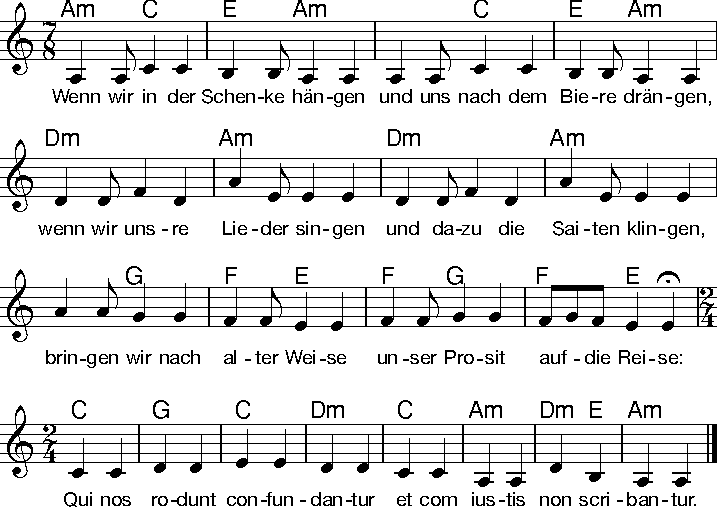
\includegraphics[width=1\textwidth]{Noten/Lied097a.pdf}

\beginverse
\[Am]Allen, \[C]die vom \[E]Wind ge\[Am]trieben, Fahrten, \[C]Land und \[E]Leute \[Am]lieben,
\[Dm]die des Nachts in \[Am]Hecken schlafen, \[Dm]wo sich Fuchs und \[Am]Hase trafen,
jedem \[G]Burschen \[F]gilt die \[E]Runde, \[F]doch den \[G]Spießern \[F]diese \[E]Kunde:
\endverse

\beginchorus
\[C]Qui nos \[G]rodunt \[C]confun\[Dm]dantur \[C]et cum \[Am]iustis \[Dm]non \[E]scri\[Am]bantur.
\endchorus
 
\beginverse
^Sein es ^Ritter ^oder ^Knappen mit Ba^rett und ^and'ren ^Kappen,
^ob in Wämsen ^oder Hemden, ^den Bekannten ^wie den Fremden
tut Be^scheid mit ^vollem ^Glase, ^hoch das ^Leben, ^hoch die ^Nase!
\endverse
%\renewcommand{\everychorus}{\textnote{\bf Refrain (wdh.)}}


\beginchorus
\[C]Qui nos \[G]rodunt \[C]confun\[Dm]dantur \[C]et cum \[Am]iustis \[Dm]non \[E]scri\[Am]bantur.
\endchorus

\beginverse
^Einer ^muss die ^Zeche ^zahlen, Tanta^lus in ^seinen ^Qualen
^hätte gern den ^vollen Becher, ^hurtig denn ihr ^frohen Zecher,
lasst uns ^diese ^Nacht ge^nießen, ^da noch ^alle ^Quellen ^fließen.
\endverse


\beginchorus
\[C]Qui nos \[G]rodunt \[C]confun\[Dm]dantur \[C]et cum \[Am]iustis \[Dm]non \[E]scri\[Am]bantur.
\endchorus

\beginverse
^Soll der ^Gersten^saft uns ^munden, Wander^vögeln, ^schrägen ^Kunden,
^Schwartenhälsen ^und Vaganten, ^Wasser lasst den ^alten Tanten
und auch ^den Ka^millen^tee, ^sehr zum ^Wohle! ^Prost! ^Olé!
\endverse

\beginchorus
\[C]Qui nos \[G]rodunt \[C]confun\[Dm]dantur \[C]et cum \[Am]iustis \[Dm]non \[E]scri\[Am]bantur.
\endchorus

\endsong

\beginscripture{}
Qui nos rodunt... (aus der Carmina Burana) = Wer uns lacht, wird unkenntlich gemacht und nicht zusammen mit den Gerechten verzeichnet.
\endscripture